\documentclass[a4paper,12pt,italian,towside]{article}
\usepackage[latin1]{inputenc}
% Comment the following line to deny the usage of umlauts and other non-ASCII characters
\usepackage[italian]{babel}

%pack per link
\usepackage{hyperref}
\hypersetup{colorlinks=true,linkcolor=blue}

%pack per colori
\usepackage{xcolor}

%pack tabelle
\usepackage{graphicx}

% Uncomment the following line to allow the usage of graphics (.jpg, .png, etc.)
\usepackage{graphicx}

\setcounter{tocdepth}{3}

%titolo e autore
\title{Progettazione Base di Dati}
\author{Francesco Luca Piero Giovanni}
\date{}

%intestazioni e pie pagina
\usepackage{fancyhdr}
\pagestyle{fancy}
\chead{}
\cfoot{\thepage}
\lhead{}
\renewcommand{\headrulewidth}{0.4pt}


%*************************************************************************%
% Start the document
\begin{document}


%generiamo il titolo
\maketitle
\newpage

%indice
\tableofcontents

\newpage
% *****sezione1*****
\section{Descrizione del progetto}
Si vuole realizzare una base di dati per modellare correttamete i Corsi di Caurea dell'Universit\'a di Padova.
Si vogliono rappresentare tutti i dati funzionali ai Corso di Laurea come Scuole, Classi, Curriculum, Attivit\'a formative e relativi SSD, Coorti, Percorsi e Docenti.
In questo progetto non vengono coinvolti studenti o piani di studio.
\par
La modellazione viene fatta coerentemente al sito  \href{https://didattica.unipd.it/}{didattica.unipd.it}, fonte partanto di tutti i requisiti del progetto.



\subsection{Requisiti strutturati}

\textbf{Scuola}
\par Le Scuole hanno funzioni di coordinamento e di razionalizzazione delle attivit\'a didattiche, compresa la proposta di istituzione, attivazione, modifica, disattivazione o soppressione di corsi di laurea, nonch\'e di gestione dei servizi comuni.\textcolor{red!50}{Ogni Scuola pu\'o attivare diversi corsi di laurea in linea con il settore accademico di interesse.}
\newline

\textbf{Classe}
\par
\textcolor{red!50}{Le Classi sono dei contenitori che raggruppano i corsi di studio dello stesso ciclo, comunque denominati dagli Atenei, aventi gli stessi obiettivi formativi qualificanti e attivit\'a formative attivate per un numero di crediti e in settori individuati come indispensabili. Le caratteristiche delle Classi sono fissate a livello nazionale, con appositi Decreti Ministeriali, e sono quindi comuni a tutti gli atenei.I corsi di laurea appartenenti alla stessa Classe hanno identico valore legale.}
\\

\textbf{Corso di Laurea}
\par
\textcolor{red!50} { I Corsi di Laure sono l'insieme di tutte le attivit\'a formative, obbligatorie e non, proposte da un ateneo per conseguire la laurea. La laurea rilasciata \'e coerente al Corso di Laurea scelto. I Corsi di Laurea sono inquadrati in Classi ministeriali, possono prvedere pi� percorsi e afferiscono a una scuola. Per il conseguimento della Laurea, e quindi il completamento del relativo corso, lo studente deve conseguire un numero prefissato di CFU (180 per le lauree triennali). Ogni corso di Laurea appartiene ad un ordinamento legislativo che ne definisce la struttura e la valiidit� legale. Ogni Corso di Laurea pu\'o avere, a driscrezione della Suola, pi\'u Curricula.
} 
\\
\\
\\


\textbf{Curriculum}
\par
\textcolor{red!50} { Un Curriculum � una denominazione di un Corso di Laurea che ne definisce gli obbiettivi oltre che a diffirenziare lo stesso in un insieme di attivit\'a formative differenti. Pi� studenti possono dunque conseguire la stessa larea con percorsi alternativi a seconda dei loro interessi e attitudini scegliendo, ad esempio, un Curriculum Generale piuttosto che un Curriculum Applicativo.
} 
\\


\textbf{Attivit\'a Formativa}
\par
\textcolor{red!50} {Le Attivit\'a Formative sono il cuore di un Corso di Laure e rappresentano tutti gli step che uno studente deve superare per conseguire la Laurea. Esse possono essere: Tirocinio, Lingua, Prova Finale e Insegnamenti. Ogni attivit\'a� formativa si inserisce in un Corso di Laurea in un anno (I, II, II IV o V a seconda del tipo di Laurea) e in un semestre ( I o II). Ogni Attivit\'a Formativa \'e riferita a un Docente responsabile che ha il compito di definirla in termini di: tipo di valutazione, prerequisiti, conoscenze e abilit\'a da acquisire, modalit\'a di esame, criterio di valutazione, contenuti, attivit\'a, materiali, testi consigliati e lingua di emissione. Ogni Attivit\'a formativa si riferisce poi a un Dipartimento some sede fisica delle lezioni. Infine ogni Attivit\'a formativa  legata a uno o pi\'u SSD dai quali, al conseguimento da parte dello studente dell' esame, vengono rilasciati CFU. Le Attivit\'a Formative sono sono soggette a vincoli, decisi dalla Scuola, in termini di superamento di altre Attivit\'a formative precedenti.
} 
\\

\textbf{Docente}
\par
\textcolor{red!50} { I Docenti sono gli attuatori di un Attivit\'a Formativa. Piu Docenti possono essere coinvolti in una stessaAttivit\'a Formativa con ruoli differenti. Dei Docenti coinvolti di un Attivit\'a, uno e uno solo � il Responsabile della stessa e ha il compito di definirla come descritto dal paragrafo Attivit\'a formativa. Dei docenti si vogliono poi poter conoscere tutti i dati relativi ai contatti e agli ambiti di ricerca. Ogni docente pu� partecipare a pi� attivit� formative.
} 
\\




\subsection{Operazioni sulle basi di dati}

Your text goes here...

\subsection{Glossario}
Your text goes here...



\begin{table}[]
	\resizebox{\textwidth}{!}{%
		\begin{tabular}{llll}
			\hline
			\multicolumn{1}{c}{\textbf{Termine}} & \multicolumn{1}{c}{\textbf{Descrizione}}                                                                 & \multicolumn{1}{c}{\textbf{Sinonimi}} & \multicolumn{1}{c}{\textbf{Collegamenti}}                                                                     \\ \hline
			Corso di  Laurea                     & \begin{tabular}[c]{@{}l@{}}insieme di tutte le attivita formative \\ necessarie a Laurearsi\end{tabular} & Corso di studi                        & \begin{tabular}[c]{@{}l@{}}Scuola, Classe, \\ Attivit\textbackslash{}'a formativa, \\ Curriculum\end{tabular} \\ \hline
			Curriculum                           &                                                                                                          &                                       &                                                                                                               \\ \hline
			Attivit\textbackslash{}'a formativa  &                                                                                                          & Insegnamento                          &                                                                                                               \\ \hline
			SSD                                  &                                                                                                          &                                       &                                                                                                               \\ \hline
			CFU                                  &                                                                                                          &                                       &                                                                                                              
		\end{tabular}%
	}
\end{table}



\newpage

% *****sezione2*****
\section{Progettazione concettuale}
Di seguito lo schema concettuale prodotto per la rappresentazione della realt`a di interesse:

\begin{figure}
	\caption{Schema E-R completo}
	\begin{center}
		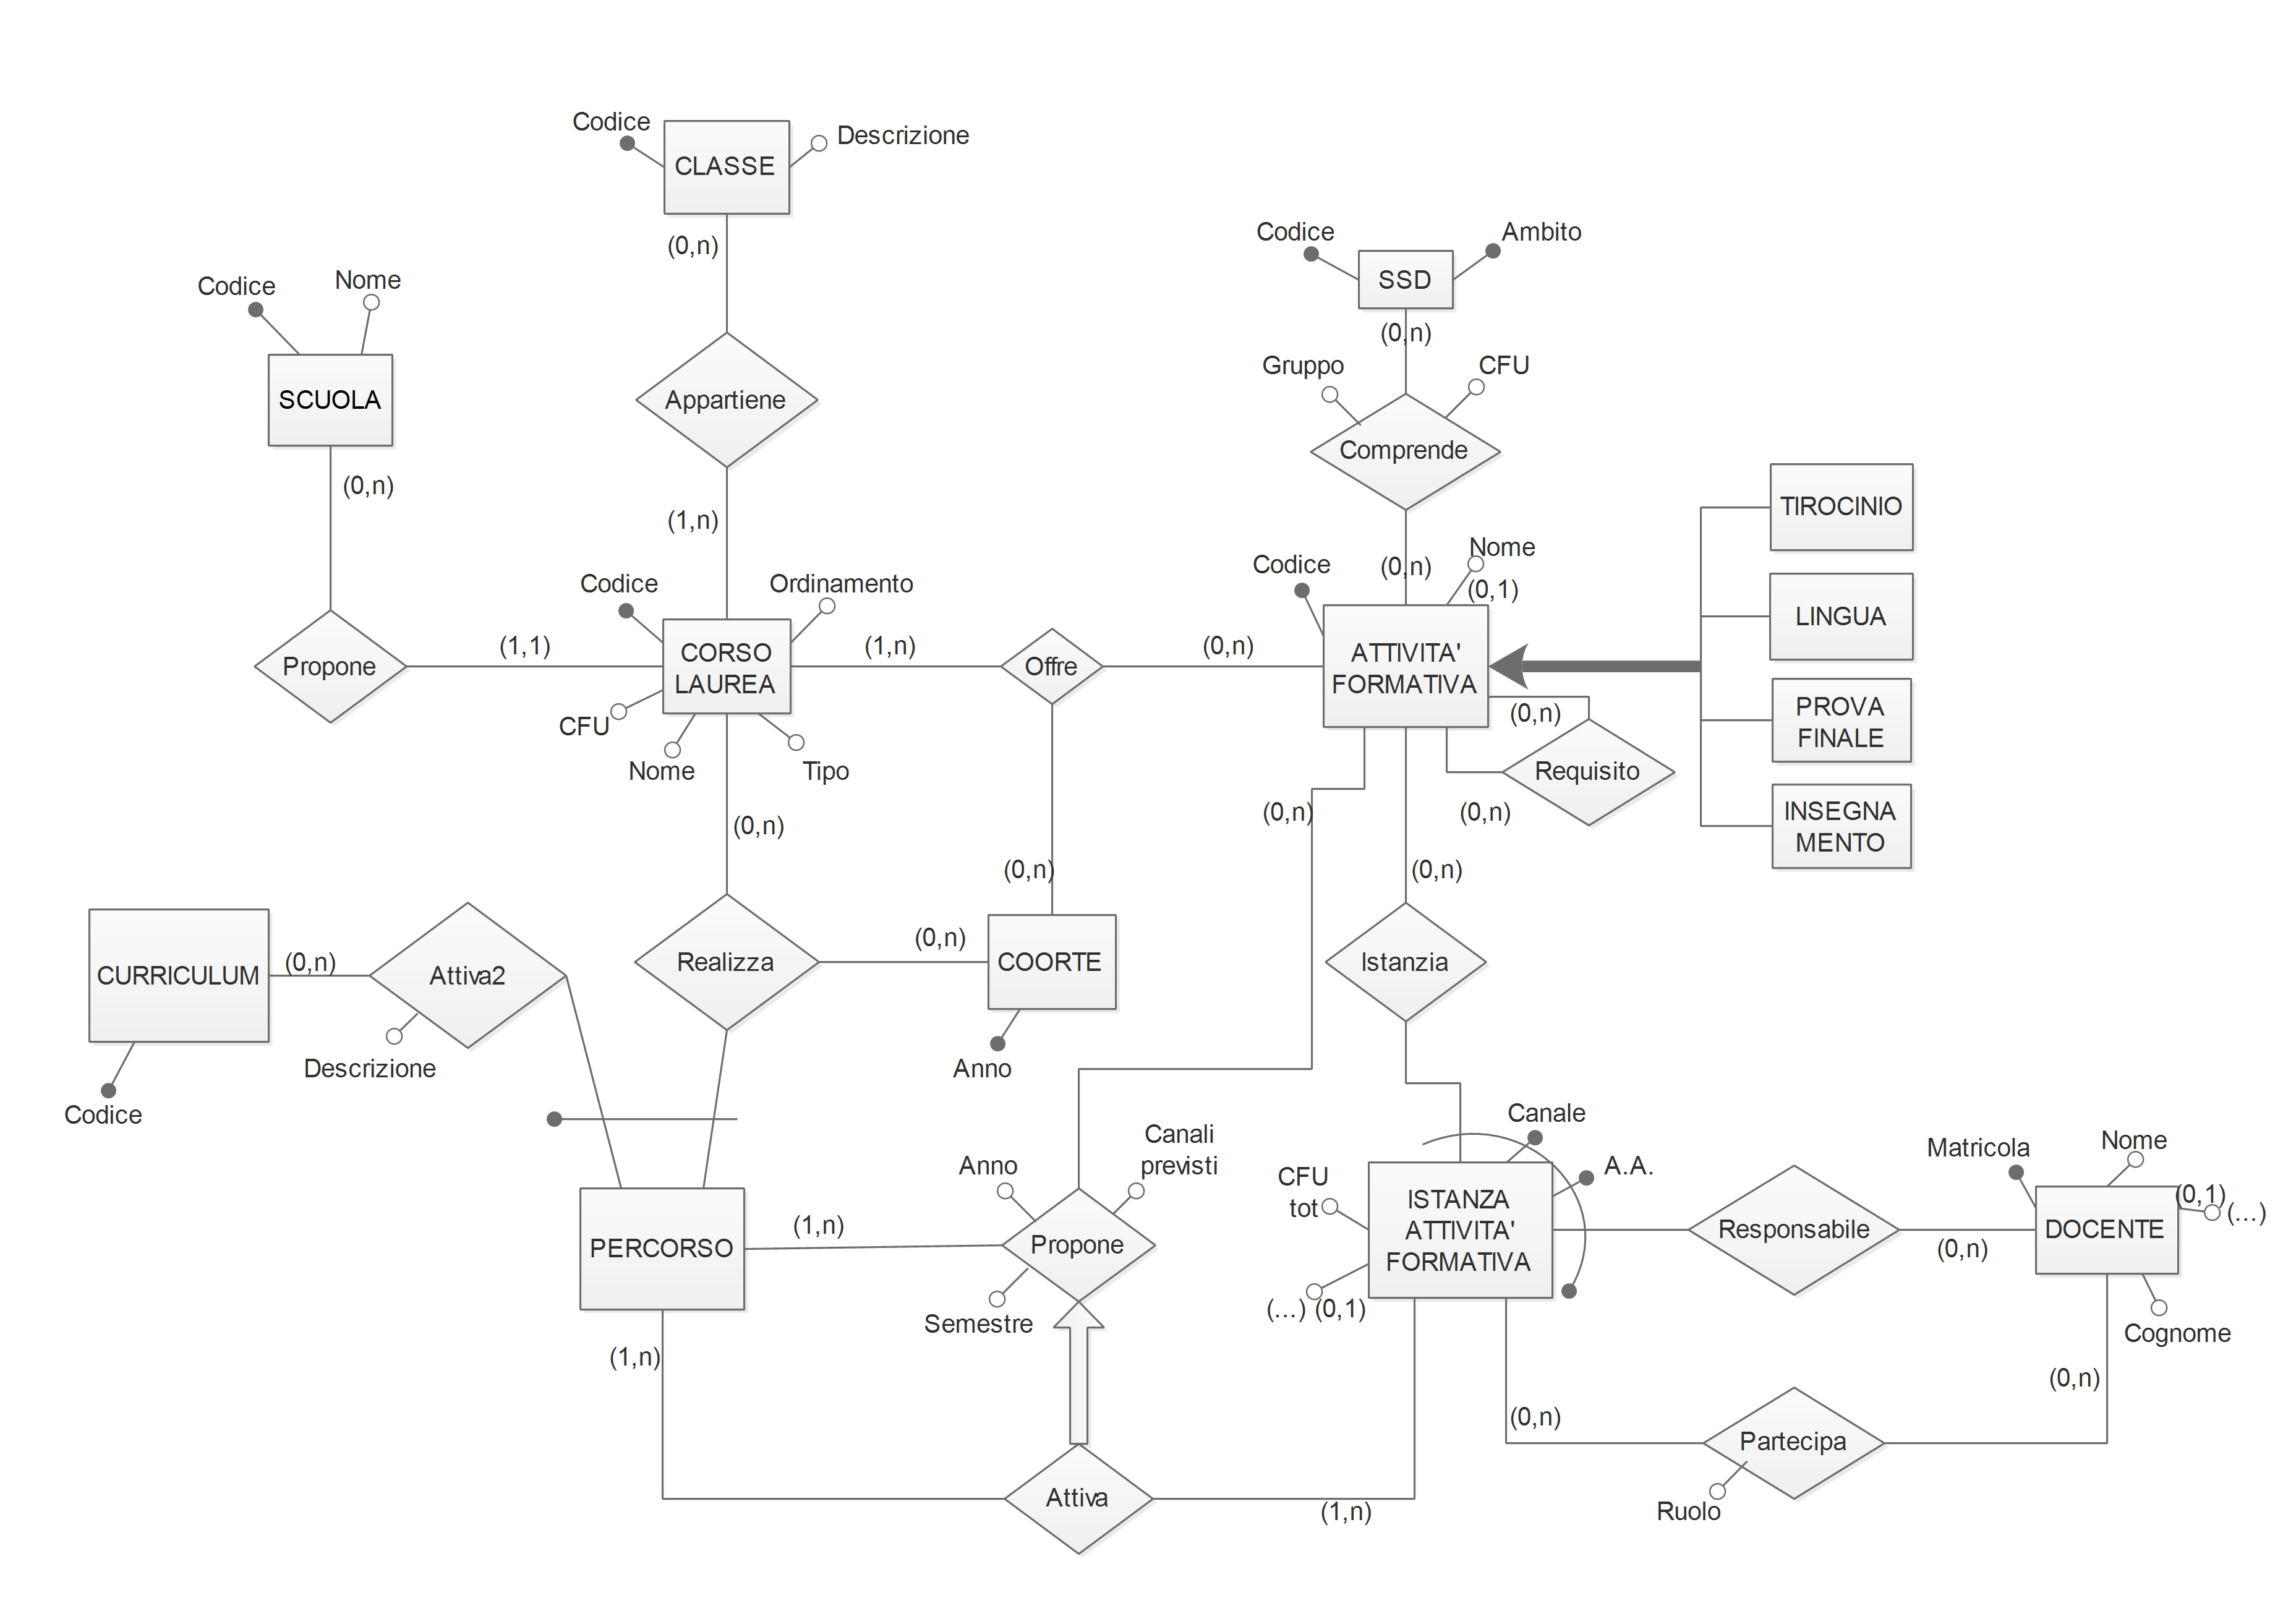
\includegraphics[]{ER diagram.jpg}
	\end{center}
\end{figure}

\subsection{Modello concettuale: Entit\`a-Associazione(E-R)}

Your text goes here...

\subsection{Dizionario dei dati}

Your text goes here...

\subsubsection{Entit\`a}

Your text goes here...

\subsubsection{Associzioni}

Your text goes here...

\subsection{Schema concettuale, regole di vincolo}

Your text goes here...
\newpage
% *****sezione3****
\section{Progettazione logica}

\subsection{Ristrutturazione schema E-R}

Your text goes here...

\subsection{Modello logico: Relazionale}

Your text goes here...

\subsection{Schema logico e regole di vincolo}

Your text goes here...
\newpage
% *****sezione4****
\section{SQL}

Your text goes here...

\subsection{Struttura}

Your text goes here...

\subsection{Query}

Your text goes here...
\newpage
% *****sezione 5*****

\section{Note}

Your text goes here...


% Uncomment the following two lines if you want to have a bibliography. Please do not forget to add an entry to your bibliography and reference it by using the \cite{} command
%\bibliographystyle{alphadin}
%\bibliography{document}

% End of the document
\end{document}